%%%%%%%%%%%%%%%%%%%%%%%%%%%%%%%%%%%%%%%%%%%%%%%%%%%%%%%%%%%%%%%%%%%%%%%%%%%%%%%%%
% Template: Article
%
% Por: Abrantes Araújo Silva Filho
%      abrantesasf@gmail.com
%
% Citação: Se você gostou deste template, por favor ajude a divulgá-lo mantendo
%          o link para meu repositório GitHub em:
%          https://github.com/abrantesasf/LaTeX
%%%%%%%%%%%%%%%%%%%%%%%%%%%%%%%%%%%%%%%%%%%%%%%%%%%%%%%%%%%%%%%%%%%%%%%%%%%%%%%%%




%%%%%%%%%%%%%%%%%%%%%%%%%%%%%%%%%%%%%%%%%%%%%%%%%%%%%%%%%%%%%%%%%%%%%%%%%%%%%%%%%
%%% Configura o tipo de documento, papel, tamanho da fonte e informações básicas
%%% para as proriedades do PDF/DVIPS e outras propriedades do documento
\RequirePackage{ifpdf}
\ifpdf
  % Classe, língua e tamanho da fonte padrão. Outras opções a considerar:
  %   draft
  %   onecolumn (padrão) ou twocolumn (OU usar o package multicol)
  %   fleqn com ou sem leqno (alinhamento à esquerda das fórmulas e dos números)
  %   oneside (padrão para article ou report) ou twoside (padrão para book)
  \documentclass[pdftex, brazil, 12pt, twoside]{article}
\else
  % Classe, língua e tamanho da fonte padrão. Outras opções a considerar:
  %   draft
  %   onecolumn (padrão) ou twocolumn (OU usar o package multicol)
  %   fleqn com ou sem leqno (alinhamento à esquerda das fórmulas e dos números)
  %   oneside (padrão para article ou report) ou twoside (padrão para book)
  \documentclass[brazil, 12pt]{article}
\fi


%%%%%%%%%%%%%%%%%%%%%%%%%%%%%%%%%%%%%%%%%%%%%%%%%%%%%%%%%%%%%%%%%%%%%%%%%%%%%%%%%
%%% Carrega pacotes iniciais necessários para estrutura de controle e para a
%%% criação e o parse de novos comandos
\usepackage{ifthen}
\usepackage{xparse}


%%%%%%%%%%%%%%%%%%%%%%%%%%%%%%%%%%%%%%%%%%%%%%%%%%%%%%%%%%%%%%%%%%%%%%%%%%%%%%%%%
%%% Configuração do tamanho da página, margens, espaçamento entrelinhas e, se
%%% necessário, ativa a indentação dos primeiros parágrafos.
\ifpdf
  \usepackage[pdftex]{geometry}
\else
  \usepackage[dvips]{geometry}
\fi
\geometry{a4paper, left=2.6cm, right=4.0cm, top=3.0cm, bottom=3.4cm}

\usepackage{setspace}
  \singlespacing
  %\onehalfspacing
  %\doublespacing


%%%%%%%%%%%%%%%%%%%%%%%%%%%%%%%%%%%%%%%%%%%%%%%%%%%%%%%%%%%%%%%%%%%%%%%%%%%%%%%%%
%%% Configurações de cabeçalho e rodapé:
\usepackage{fancyhdr}
\setlength{\headheight}{1cm}
\setlength{\footskip}{1.5cm}
\renewcommand{\headrulewidth}{0.3pt}
\renewcommand{\footrulewidth}{0.0pt}
\pagestyle{fancy}
\renewcommand{\sectionmark}[1]{%
  \markboth{\uppercase{#1}}{}}
\renewcommand{\subsectionmark}[1]{%
  \markright{\uppercase{\thesubsection \hspace{0.1cm} #1}}{}}
\fancyhead{}
\fancyfoot{}
\newcommand{\diminuifonte}{%
    \fontsize{9pt}{9}\selectfont
}
\newcommand{\aumentafonte}{%
    \fontsize{12}{12}\selectfont
}
% Configura cabeçalho e rodapé para documentos TWOSIDE
\fancyhead[EL]{\textbf{\thepage}}
\fancyhead[EC]{}
\fancyhead[ER]{\diminuifonte \textbf{\leftmark}}
\fancyhead[OR]{\textbf{\thepage}}
\fancyhead[OC]{}
\fancyhead[OL]{\diminuifonte \textbf{\rightmark}}
\fancyfoot[EL,EC,ER,OR,OC,OL]{}
% Configura cabeçalho e rodapé para documentos ONESIDE
%\lhead{ \fancyplain{}{sup esquerdo} }
%\chead{ \fancyplain{}{sup centro} }
%\rhead{ \fancyplain{}{\thesection} }
%\lfoot{ \fancyplain{}{inf esquerdo} }
%\cfoot{ \fancyplain{}{inf centro} }
%\rfoot{ \fancyplain{}{\thepage} }




%%%%%%%%%%%%%%%%%%%%%%%%%%%%%%%%%%%%%%%%%%%%%%%%%%%%%%%%%%%%%%%%%%%%%%%%%%%%%%%%%
%%% Configurações de encoding, lingua e fontes:
\usepackage[T1]{fontenc}
\usepackage[utf8]{inputenc}
\usepackage{babel}

% Altera a fonte padrão do documento (nem todas funcionam em modo math):
%   phv = Helvetica
%   ptm = Times
%   ppl = Palatino
%   pbk = bookman
%   pag = AdobeAvantGarde
%   pnc = Adobe NewCenturySchoolBook
\renewcommand{\familydefault}{ppl}


%%%%%%%%%%%%%%%%%%%%%%%%%%%%%%%%%%%%%%%%%%%%%%%%%%%%%%%%%%%%%%%%%%%%%%%%%%%%%%%%%
%%% Carrega pacotes para referências cruzadas, citações dentro do documento,
%%% links para internet e outros.Configura algumas opções.
%%% Não altere a ordem de carregamento dos packages.
\usepackage{varioref}
\ifpdf
  \usepackage[pdftex]{hyperref}
    \hypersetup{
      % Informações variáveis em cada documento (MUDE AQUI!):
      pdftitle={Resumo de Pré-Cálculo},
      pdfauthor={Abrantes Araújo Silva Filho},
      pdfsubject={Resumo dos tópicos mais importantes de Pré-Cálculo},
      pdfkeywords={pré-cálculo, precalculus, resumo, revisão},
      pdfinfo={
        CreationDate={}, % Ex.: D:AAAAMMDDHH24MISS
        ModDate={}       % Ex.: D:AAAAMMDDHH24MISS
      },
      % Coisas que você não deve alterar se não souber o que está fazendo:
      unicode=true,
      pdflang={pt-BR},
      bookmarksopen=true,
      bookmarksnumbered=true,
      bookmarksopenlevel=5,
      pdfdisplaydoctitle=true,
      pdfpagemode=UseOutlines,
      pdfstartview=FitH,
      pdfcreator={LaTeX with hyperref package},
      pdfproducer={pdfTeX},
      pdfnewwindow=true,
      colorlinks=true,
      citecolor=green,
      linkcolor=red,
      filecolor=cyan,
      urlcolor=blue
    }
\else
  \usepackage{hyperref}
\fi
\usepackage{cleveref}
\usepackage{url}


%%%%%%%%%%%%%%%%%%%%%%%%%%%%%%%%%%%%%%%%%%%%%%%%%%%%%%%%%%%%%%%%%%%%%%%%%%%%%%%%%
%%% Carrega bibliotecas de símbolos (matemáticos, físicos, etc.), fontes
%%% adicionais, e configura algumas opções
\usepackage{amsmath}
\usepackage{amssymb}
\usepackage{amsfonts}
\usepackage{siunitx}
  \sisetup{group-separator = {.}}
  \sisetup{group-digits = {false}}
  \sisetup{output-decimal-marker = {,}}
\usepackage{bm}
\usepackage{cancel}
% Altera separador decimal via comando, se necessário (prefira o siunitx):
%\mathchardef\period=\mathcode`.
%\DeclareMathSymbol{.}{\mathord}{letters}{"3B}
  

%%%%%%%%%%%%%%%%%%%%%%%%%%%%%%%%%%%%%%%%%%%%%%%%%%%%%%%%%%%%%%%%%%%%%%%%%%%%%%%%%
%%% Carrega packages relacionados à computação
\usepackage{algorithm2e}
\usepackage{algorithmicx}
\usepackage{algpseudocode}
\usepackage{listings}
  \lstset{literate=
    {á}{{\'a}}1 {é}{{\'e}}1 {í}{{\'i}}1 {ó}{{\'o}}1 {ú}{{\'u}}1
    {Á}{{\'A}}1 {É}{{\'E}}1 {Í}{{\'I}}1 {Ó}{{\'O}}1 {Ú}{{\'U}}1
    {à}{{\`a}}1 {è}{{\`e}}1 {ì}{{\`i}}1 {ò}{{\`o}}1 {ù}{{\`u}}1
    {À}{{\`A}}1 {È}{{\'E}}1 {Ì}{{\`I}}1 {Ò}{{\`O}}1 {Ù}{{\`U}}1
    {ä}{{\"a}}1 {ë}{{\"e}}1 {ï}{{\"i}}1 {ö}{{\"o}}1 {ü}{{\"u}}1
    {Ä}{{\"A}}1 {Ë}{{\"E}}1 {Ï}{{\"I}}1 {Ö}{{\"O}}1 {Ü}{{\"U}}1
    {â}{{\^a}}1 {ê}{{\^e}}1 {î}{{\^i}}1 {ô}{{\^o}}1 {û}{{\^u}}1
    {Â}{{\^A}}1 {Ê}{{\^E}}1 {Î}{{\^I}}1 {Ô}{{\^O}}1 {Û}{{\^U}}1
    {œ}{{\oe}}1 {Œ}{{\OE}}1 {æ}{{\ae}}1 {Æ}{{\AE}}1 {ß}{{\ss}}1
    {ű}{{\H{u}}}1 {Ű}{{\H{U}}}1 {ő}{{\H{o}}}1 {Ő}{{\H{O}}}1
    {ç}{{\c c}}1 {Ç}{{\c C}}1 {ø}{{\o}}1 {å}{{\r a}}1 {Å}{{\r A}}1
    {€}{{\euro}}1 {£}{{\pounds}}1 {«}{{\guillemotleft}}1
    {»}{{\guillemotright}}1 {ñ}{{\~n}}1 {Ñ}{{\~N}}1 {¿}{{?`}}1
  }
  

%%%%%%%%%%%%%%%%%%%%%%%%%%%%%%%%%%%%%%%%%%%%%%%%%%%%%%%%%%%%%%%%%%%%%%%%%%%%%%%%%
%%% Ativa suporte extendido a cores
\usepackage[svgnames]{xcolor} % Opções de cores: usenames (16), dvipsnames (64),
                              % svgnames (150) e x11names (300).


%%%%%%%%%%%%%%%%%%%%%%%%%%%%%%%%%%%%%%%%%%%%%%%%%%%%%%%%%%%%%%%%%%%%%%%%%%%%%%%%%
%%% Suporte à importação de gráficos externos
\ifpdf
  \usepackage[pdftex]{graphicx}
\else
  \usepackage[dvips]{graphicx}
\fi


%%%%%%%%%%%%%%%%%%%%%%%%%%%%%%%%%%%%%%%%%%%%%%%%%%%%%%%%%%%%%%%%%%%%%%%%%%%%%%%%%
%%% Suporte à criação de gráficos proceduralmente na LaTeX:
\usepackage{tikz}
  \usetikzlibrary{arrows,automata,backgrounds,matrix,patterns,positioning,shapes,shadows}


%%%%%%%%%%%%%%%%%%%%%%%%%%%%%%%%%%%%%%%%%%%%%%%%%%%%%%%%%%%%%%%%%%%%%%%%%%%%%%%%%
%%% Packages para tabelas
\usepackage{array}
\usepackage{longtable}
\usepackage{tabularx}
\usepackage{tabu}
\usepackage{lscape}
\usepackage{colortbl}  
\usepackage{booktabs}


%%%%%%%%%%%%%%%%%%%%%%%%%%%%%%%%%%%%%%%%%%%%%%%%%%%%%%%%%%%%%%%%%%%%%%%%%%%%%%%%%
%%% Packages ambientes de listas
\usepackage{enumitem}
\usepackage[ampersand]{easylist}


%%%%%%%%%%%%%%%%%%%%%%%%%%%%%%%%%%%%%%%%%%%%%%%%%%%%%%%%%%%%%%%%%%%%%%%%%%%%%%%%%
%%% Packages para suporte a ambientes floats, captions, etc.:
\usepackage{float}
\usepackage{wrapfig}
\usepackage{placeins}
\usepackage{caption}
\usepackage{sidecap}
\usepackage{subcaption}


%%%%%%%%%%%%%%%%%%%%%%%%%%%%%%%%%%%%%%%%%%%%%%%%%%%%%%%%%%%%%%%%%%%%%%%%%%%%%%%%%
%%% Meus comandos específicos:
% Commando para ``italizar´´ palavras em inglês (e outras línguas!):
\newcommand{\ingles}[1]{\textit{#1}}

% Commando para colocar o espaço correto entre um número e sua unidade:
\newcommand{\unidade}[2]{\ensuremath{#1\,\mathrm{#2}}}
\newcommand{\unidado}[2]{{#1}\,{#2}}

% Produz ordinal masculino ou feminino dependendo do segundo argumento:
\newcommand{\ordinal}[2]{%
#1%
\ifthenelse{\equal{a}{#2}}%
{\textordfeminine}%
{\textordmasculine}}


%%%%%%%%%%%%%%%%%%%%%%%%%%%%%%%%%%%%%%%%%%%%%%%%%%%%%%%%%%%%%%%%%%%%%%%%%%%%%%%%%
%%% Hifenização específica quando o LaTeX/Babel não conseguirem hifenizar:
\babelhyphenation{Git-Hub}


%%%%%%%%%%%%%%%%%%%%%%%%%%%%%%%%%%%%%%%%%%%%%%%%%%%%%%%%%%%%%%%%%%%%%%%%%%%%%%%%%
%%%%%%%%%%%%%%%%%%%%%%%%%%%%%%%%%%%%%%%%%%%%%%%%%%%%%%%%%%%%%%%%%%%%%%%%%%%%%%%%%
%%%%%%%%%%%%%%%%%%%%%%%%%%%%%%%%%%%%%%%%%%%%%%%%%%%%%%%%%%%%%%%%%%%%%%%%%%%%%%%%%
%%%%%%%%%%%%%%%%%%%%%%%%%%%%%%%%%%%%%%%%%%%%%%%%%%%%%%%%%%%%%%%%%%%%%%%%%%%%%%%%%
%%%%%%%%%%%%%%%%%%%%%%%%%%%%%% COMEÇA O DOCUMENTO %%%%%%%%%%%%%%%%%%%%%%%%%%%%%%%
%%%%%%%%%%%%%%%%%%%%%%%%%%%%%%%%%%%%%%%%%%%%%%%%%%%%%%%%%%%%%%%%%%%%%%%%%%%%%%%%%
%%%%%%%%%%%%%%%%%%%%%%%%%%%%%%%%%%%%%%%%%%%%%%%%%%%%%%%%%%%%%%%%%%%%%%%%%%%%%%%%%
%%%%%%%%%%%%%%%%%%%%%%%%%%%%%%%%%%%%%%%%%%%%%%%%%%%%%%%%%%%%%%%%%%%%%%%%%%%%%%%%%
%%%%%%%%%%%%%%%%%%%%%%%%%%%%%%%%%%%%%%%%%%%%%%%%%%%%%%%%%%%%%%%%%%%%%%%%%%%%%%%%%
\begin{document}
\title{Resumo de Pré-Cálculo}
\author{Abrantes Araújo Silva Filho}
\date{2018-07-23}
\maketitle
\tableofcontents
\newpage

%%%%%%%%%%%%%%%%%%%%%%%%%%%%%%%%%%%%%%%%%%%%%%%%%%%%%%%%%%%%%%%%%%%%%%%%%%%%%%%%%
%%%%%%%%%%%%%%%%%%%%%%%%%%%%%%%%%%%%%%%%%%%%%%%%%%%%%%%%%%%%%%%%%%%%%%%%%%%%%%%%%
%%%%%%%%%%%%%%%%%%%%%%%%%%%%%%%%%%%%%%%%%%%%%%%%%%%%%%%%%%%%%%%%%%%%%%%%%%%%%%%%%
\section{Introdução}
\label{intro}

Este documento é um resumo de \emph{Pré-Cálculo} que preparei durante o mês de julho
de 2018, como estudo prévio para as disciplinas de ``Cálculo Diferencial e Integral I''
e ``Álgebra Linear e Geometria Analítica'', do curso de
\href{https://www.faesa.br/curso/ciencia-da-computacao/}{Ciência da Computação}
da \href{https://www.faesa.br/}{FAESA Centro Universitário}.

A FAESA não oferece um curso de Pré-Cálculo em sua grade de disciplinas, nem indica
materiais de referência para estudo. Então, após algumas pesquisas na internet,
resolvi utilizar os seguintes materiais para estudo:

\begin{itemize}
\item \textbf{Collingwood DH, Prince KD, Conroy MM. \emph{Precalculus}. Seattle (WA): University
  of Washington, 2017.}

  Este é o livro texto adotado pelos professores da disciplina
  ``Math 120 - Precalculus'', da University of Washington, e está disponível para
  acesso e download público no \href{https://sites.math.washington.edu/~m120/}{site da disciplina}.
  Nesse site estão disponíveis, além do livro, diversos outros materiais de auxílio ao aprendizado
  de pré-cálculo, como exercícios corrigidos, provas corrigidas e outros.
  
\item \textbf{Simmons GF. \emph{Precalculus Mathematics in a Nutshell: Geometry, Algebra, Trigonometry}. New
  York: Wipf and Stock Publishers, 2003.}

  Este livro está disponível para empréstimo on-line
  no \href{https://archive.org/details/precalculusmathe00geor}{Internet Archive} ou
  aquisição na \href{https://www.amazon.com/Precalculus-Mathematics-Nutshell-Geometry-Trigonometry/dp/1592441300/}{Amazon}.
  É um livro bem objetivo e pequeno, mas com boa avaliação pelos leitores.
\end{itemize}

As seguintes ferramentas também foram importantes para o estudo (principalmente para
ajudar na álgebra):
\begin{itemize}[noitemsep]
\item \href{http://www.wolframalpha.com/}{Wolfram|Alpha}
\item \href{https://www.geogebra.org/}{GeoGebra}
\item \href{https://www.symbolab.com/}{Symbolab}
\item \href{https://photomath.net/}{Photomat}
\end{itemize}

ATENÇÃO: nenhum texto aqui é de minha autoria! Eu apenas resumi e retirei das fontes anteriormente
citadas os principais conceitos de pré-cálculo para meu próprio estudo. Todo o crédito pertence
aos autores originais!


%%%%%%%%%%%%%%%%%%%%%%%%%%%%%%%%%%%%%%%%%%%%%%%%%%%%%%%%%%%%%%%%%%%%%%%%%%%%%%%%%
%%%%%%%%%%%%%%%%%%%%%%%%%%%%%%%%%%%%%%%%%%%%%%%%%%%%%%%%%%%%%%%%%%%%%%%%%%%%%%%%%
%%%%%%%%%%%%%%%%%%%%%%%%%%%%%%%%%%%%%%%%%%%%%%%%%%%%%%%%%%%%%%%%%%%%%%%%%%%%%%%%%
\section{Notas e orientações iniciais}
\label{notas}

%%%%%%%%%%%%%%%%%%%%%%%%%%%%%%%%%%%%%%%%%%%%%%%%%%%%%%%%%%%%%%%%%%%%%%%%%%%%%%%%%
%%%%%%%%%%%%%%%%%%%%%%%%%%%%%%%%%%%%%%%%%%%%%%%%%%%%%%%%%%%%%%%%%%%%%%%%%%%%%%%%%
\subsection{Por que estudar pré-cálculo?}
\label{notas-por-que}

Porque em praticamente todas as áreas da ciência a matemática
tornou-se a lingua básica para a troca de informações e o pré-cálculo é a porta de entrada
para o entendimento mais avançado da matemática (cálculo, etc.).

O difícil no pré-cálculo (cálculo, álgebra linear, etc.) não é nem a matemática em
si mesma, é a \emph{interpretação} de um problema que está expresso em palavras. Você
deve: 1) ler; 2) entender; 3) pensar; 4) relacionar conceitos; 5) esquematizar figuras;
6) investir tempo; e, somente no fim, 7) escolher fórmulas e contas para resolver o
problema.

Note como o grosso do processo é a \emph{interpretação} do problema, não o cálculo
da resposta em si.

%%%%%%%%%%%%%%%%%%%%%%%%%%%%%%%%%%%%%%%%%%%%%%%%%%%%%%%%%%%%%%%%%%%%%%%%%%%%%%%%%
%%%%%%%%%%%%%%%%%%%%%%%%%%%%%%%%%%%%%%%%%%%%%%%%%%%%%%%%%%%%%%%%%%%%%%%%%%%%%%%%%
\subsection{Os principais erros}
\label{notas-principais-erros}

Os principais erros ao se resolver problemas matemáticos do nível de pré-cálculo
(ou superiores) são:

\begin{itemize}
\item \textbf{Álgebra}: aqui é que a maioria se perde. Não conhecer as regras de
  manipulação algébrica garante horas e horas de frustração.
\item \textbf{Visualização}: se você não desenhar um rascunho do problema, com
  figuras e indicações do que está ocorrendo, você não conseguirá resolver o problema
  ou gastará horas a mais do que o necessário.
\item \textbf{Definições}: se você não souber as definições matemáticas envolvidas
  no problema, não conseguirá resolvê-lo.
\end{itemize}

%%%%%%%%%%%%%%%%%%%%%%%%%%%%%%%%%%%%%%%%%%%%%%%%%%%%%%%%%%%%%%%%%%%%%%%%%%%%%%%%%
%%%%%%%%%%%%%%%%%%%%%%%%%%%%%%%%%%%%%%%%%%%%%%%%%%%%%%%%%%%%%%%%%%%%%%%%%%%%%%%%%
\subsection{Como resolver um problema?}
\label{notas-como-resolver}

Nunca passe diretamente do \emph{texto} do problema para a sua representação
\emph{simbólica} (fórmulas, equações, variáveis, etc.). Sempre faça uma
\emph{visualização} do problema e, depois de ter certeza que entendeu tudo,
aí sim você começa a representá-lo simbolicamente para resolvê-lo.

\begin{figure}[ht]
  \begin{center}
    \caption{De palavras para figuras e depois para símbolos}
    \label{fig:palavras-imagens-simbolos}
    %\fbox{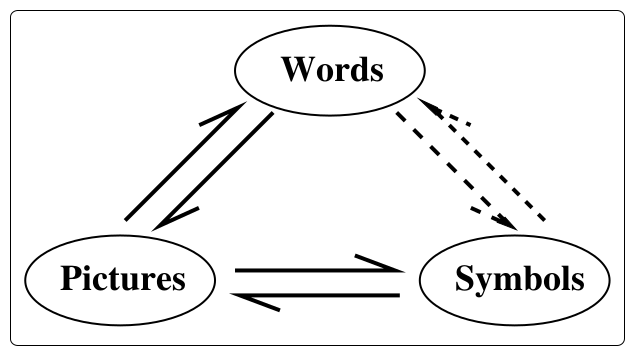
\includegraphics[scale=0.5]{imagens/palavras-imagens-simbolos.png}}
    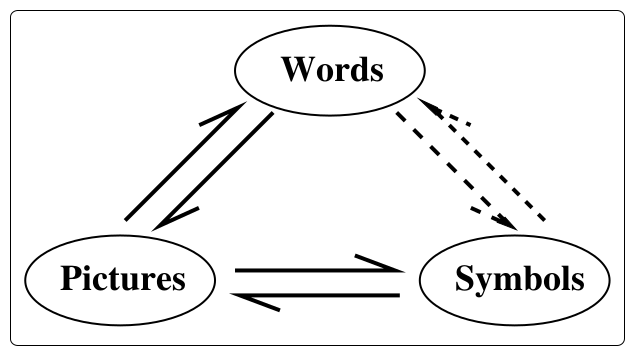
\includegraphics[scale=0.5]{imagens/palavras-imagens-simbolos.png}
    
    \footnotesize{Fonte:~Collingwood DH et al. Precalculus, pág.\ x}
  \end{center}
\end{figure}


%%%%%%%%%%%%%%%%%%%%%%%%%%%%%%%%%%%%%%%%%%%%%%%%%%%%%%%%%%%%%%%%%%%%%%%%%%%%%%%%%
%%%%%%%%%%%%%%%%%%%%%%%%%%%%%%%%%%%%%%%%%%%%%%%%%%%%%%%%%%%%%%%%%%%%%%%%%%%%%%%%%
%%%%%%%%%%%%%%%%%%%%%%%%%%%%%%%%%%%%%%%%%%%%%%%%%%%%%%%%%%%%%%%%%%%%%%%%%%%%%%%%%
\section{Aquecimento}
\label{aquecimento}

%%%%%%%%%%%%%%%%%%%%%%%%%%%%%%%%%%%%%%%%%%%%%%%%%%%%%%%%%%%%%%%%%%%%%%%%%%%%%%%%%
%%%%%%%%%%%%%%%%%%%%%%%%%%%%%%%%%%%%%%%%%%%%%%%%%%%%%%%%%%%%%%%%%%%%%%%%%%%%%%%%%
\subsection{Diferença entre ``graficar'' e modelar}
\label{aquecimento-graficar-modelar}

A primeira diferença importante a ter em mente é a diferença entre ``\emph{graficar}''\footnote{Obviamente
  a palavra ``graficar'' não existe em português mas estou usando esse neologismo para substituir
  a palavra inglesa \emph{graphing} que significa plotar ou desenhar um gráfico.} e \emph{modelar}.

\begin{itemize}
\item \textbf{Graficar}: é o processo de desenhar um gráfico ou figura, a partir de equações
  ou fórmulas já definidas.
\item \textbf{Modelar}: é o processo de estabelecer equações ou fórmular, a partir de dados
  brutos ou figuras.
\end{itemize}

A modelagem é um processo muito mais difícil do que a ``graficagem''\footnote{Mesmo caso que a nota anterior.}
pois requer experiência, intuição e um certo grau de tentativa e erro.

%%%%%%%%%%%%%%%%%%%%%%%%%%%%%%%%%%%%%%%%%%%%%%%%%%%%%%%%%%%%%%%%%%%%%%%%%%%%%%%%%
%%%%%%%%%%%%%%%%%%%%%%%%%%%%%%%%%%%%%%%%%%%%%%%%%%%%%%%%%%%%%%%%%%%%%%%%%%%%%%%%%
\subsection{Números e unidades}
\label{aquecimento-numeros-unidades}

Os números não ocorrem isoladamente, geralmente são interpretados associados à alguma
\emph{unidade} de medida. Acostume-se a UTILIZAR as unidades nos cálculos, como se
fossem outro número qualquer, e manipule essas unidades exatamente como os números
(por exemplo, cancelando as unidades comuns no numerador e denominador de uma fração).

%%%%%%%%%%%%%%%%%%%%%%%%%%%%%%%%%%%%%%%%%%%%%%%%%%%%%%%%%%%%%%%%%%%%%%%%%%%%%%%%%
%%%%%%%%%%%%%%%%%%%%%%%%%%%%%%%%%%%%%%%%%%%%%%%%%%%%%%%%%%%%%%%%%%%%%%%%%%%%%%%%%
\subsection{Introdução às taxas}
\label{aquecimento-introducao-taxas}

De modo bem básico e introdutório, uma taxa corresponde à variação de uma quantidade
em relação à variação de uma outra quantidade. Por exemplo:

\begin{equation}
  \text{taxa} = \frac{\Delta\ \text{quantidade ``a''}}{\Delta\ \text{quantidade ``b''}}
\end{equation}

Geralmente o denominador de maior interesse de uma taxa é o \emph{tempo}. Assim temos
que as taxas de variação de maior interesse para nós são do tipo:

\begin{equation}
  \text{taxa} = \frac{\Delta\ \text{quantidade ``a''}}{\Delta\ \text{tempo}}
\end{equation}

Uma taxa pode ser:
\begin{itemize}
\item \textbf{Positiva} ou \textbf{Negativa}: uma quantidade está aumentando ou diminuindo
  em relação à outra;
\item \textbf{Constante} ou \textbf{Variável}: a taxa permanece, ou não, constante durante
  o tempo.
\end{itemize}

Se, e apenas se, uma taxa for constante no tempo, podemos calcular a mudança total em uma quantidade
em um período de tempo através da fórmula:

\begin{equation}
  \text{Mudança total em uma quantidade} = \text{Taxa} \times \text{Tempo}
\end{equation}

%%%%%%%%%%%%%%%%%%%%%%%%%%%%%%%%%%%%%%%%%%%%%%%%%%%%%%%%%%%%%%%%%%%%%%%%%%%%%%%%%
%%%%%%%%%%%%%%%%%%%%%%%%%%%%%%%%%%%%%%%%%%%%%%%%%%%%%%%%%%%%%%%%%%%%%%%%%%%%%%%%%
\subsection{O processo de modelagem}
\label{aquecimento-processo-modelagem}

Toda vez que precisarmos resolver um problema tentando ``descrever'' o que está
ocorrendo e ``predizer'' o que pode ocorrer, estamos envolvidos em algum
processo de modelagem.

Na modelagem nos focamos em algumas características mais importantes, descartando
as menos importantes, e tentamos descrever matematicamente o fenômeno observado
através dessas características escolhidas.


%%%%%%%%%%%%%%%%%%%%%%%%%%%%%%%%%%%%%%%%%%%%%%%%%%%%%%%%%%%%%%%%%%%%%%%%%%%%%%%%%
%%%%%%%%%%%%%%%%%%%%%%%%%%%%%%%%%%%%%%%%%%%%%%%%%%%%%%%%%%%%%%%%%%%%%%%%%%%%%%%%%
%%%%%%%%%%%%%%%%%%%%%%%%%%%%%%%%%%%%%%%%%%%%%%%%%%%%%%%%%%%%%%%%%%%%%%%%%%%%%%%%%
\section{Impondo um sistema de coordenadas}
\label{sistema-coordenadas}

%%%%%%%%%%%%%%%%%%%%%%%%%%%%%%%%%%%%%%%%%%%%%%%%%%%%%%%%%%%%%%%%%%%%%%%%%%%%%%%%%
%%%%%%%%%%%%%%%%%%%%%%%%%%%%%%%%%%%%%%%%%%%%%%%%%%%%%%%%%%%%%%%%%%%%%%%%%%%%%%%%%
\subsection{O que é um sistema de coordenadas?}
\label{sistema-coordenadas-def}

Um sistema de coordenadas nos permite localizar pontos em um espaço (bi, tri ou
multidimensional) usando números reais (dois, três ou mais números).

Em um plano nosso sistema de coordenadas será composto por 2 eixos perpendiculares
entre si (horizontal, eixo-x, e vertical, eixo-y), que se cruzam em um ponto
chamado de ORIGEM, $P_{origem} = (0, 0)$, dividindo o espaço bidimensional
em 4 quadrantes.

%%%%%%%%%%%%%%%%%%%%%%%%%%%%%%%%%%%%%%%%%%%%%%%%%%%%%%%%%%%%%%%%%%%%%%%%%%%%%%%%%
%%%%%%%%%%%%%%%%%%%%%%%%%%%%%%%%%%%%%%%%%%%%%%%%%%%%%%%%%%%%%%%%%%%%%%%%%%%%%%%%%
\subsection{Características de um sistema de coordenadas}
\label{sistema-coordenadas-caracteristicas}

Todo sistema de coordenadas tem que especificar:

\begin{itemize}[noitemsep]
\item Origem
\item Eixos
\item Unidades (dos eixos)
\item Escala (dos eixos)
\end{itemize}

A \emph{escala} dos eixos deve ser indicada sempre que o comprimento de 1 unidade em um dos
eixos for diferente do comprimento de 1 unidade no outro eixo, alterando assim o
``aspect ratio'' do gráfico.

\begin{equation}
  \text{aspect ratio} = \frac{\text{comprimento de 1 unidade no eixo vertical}}{\text{comprimento de 1 unidade no eixo horizontal}}
\end{equation}


%%%%%%%%%%%%%%%%%%%%%%%%%%%%%%%%%%%%%%%%%%%%%%%%%%%%%%%%%%%%%%%%%%%%%%%%%%%%%%%%%
%%%%%%%%%%%%%%%%%%%%%%%%%%%%%%%%%%%%%%%%%%%%%%%%%%%%%%%%%%%%%%%%%%%%%%%%%%%%%%%%%
\subsection{A imposição de sistema de coordenadas é crítica na modelagem}
\label{sistema-coordenadas-critico-modelagem}

Na modelagem, que é sair de dados brutos e visualizações para obtermos as equações
e fórmulas que descrevem um fenômeno, um passo crítico é a imposição de um sistema
de coordenadas, da melhor forma possível, para facilitar o processo.

Vários sistemas de coordenadas, com origens em diversos locais, irão funcionar
para a modelagem. O ``pulo do gato'' é escolher o sistema de coordenadas que
irá ser mais natural ao processo e facilitar a obtenção das equações e fórmulas.

%%%%%%%%%%%%%%%%%%%%%%%%%%%%%%%%%%%%%%%%%%%%%%%%%%%%%%%%%%%%%%%%%%%%%%%%%%%%%%%%%
%%%%%%%%%%%%%%%%%%%%%%%%%%%%%%%%%%%%%%%%%%%%%%%%%%%%%%%%%%%%%%%%%%%%%%%%%%%%%%%%%
\subsection{Distância no plano}
\label{sistema-coordenadas-distancia-plano}

Para saber a distância, no plano, entre um ponto $P = (x_1, y_1)$ e um ponto
$Q = (x_2, y_2)$ podemos usar o Teorema de Pitágoras e calcular a Distância Euclidiana
entre os pontos:

\begin{figure}[ht]
  \begin{center}
    \caption{Distância no plano entre dois pontos}
    \label{fig:distancia-plano}
    %\fbox{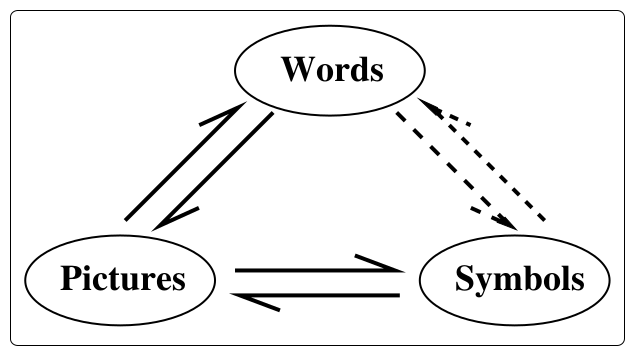
\includegraphics[scale=0.5]{imagens/palavras-imagens-simbolos.png}}
    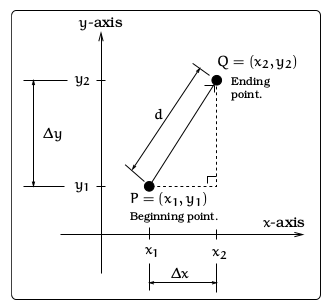
\includegraphics[scale=0.9]{imagens/distancia.png}
    
    \footnotesize{Fonte:~Collingwood DH et al. Precalculus, pág.\ 18}
  \end{center}
\end{figure}

Como os deltas podem ser negativos mas as distâncias são sempre positivas, usamos
o valor absoluto dos deltas para o cálculo. Assim temos:

\begin{equation}
  \begin{split}
    d^2 & = (|\Delta x|)^2 + (|\Delta y|)^2\\
    d^2 & = (|x_2 - x_1|)^2 + (|y_2 - y_1|)^2\\
      d & = \sqrt{(|x_2 - x_1|)^2 + (|y_2 - y_1|)^2}
  \end{split}
\end{equation}

Note também que:

\begin{itemize}[noitemsep]
\item $d$ é a distância no plano entre os pontos P e Q
\item $\Delta x$ é a distância direta no eixo x
\item $\Delta y$ é a distância direta no eixo y
\end{itemize}


%%%%%%%%%%%%%%%%%%%%%%%%%%%%%%%%%%%%%%%%%%%%%%%%%%%%%%%%%%%%%%%%%%%%%%%%%%%%%%%%%
%%%%%%%%%%%%%%%%%%%%%%%%%%%%%%%%%%%%%%%%%%%%%%%%%%%%%%%%%%%%%%%%%%%%%%%%%%%%%%%%%
%%%%%%%%%%%%%%%%%%%%%%%%%%%%%%%%%%%%%%%%%%%%%%%%%%%%%%%%%%%%%%%%%%%%%%%%%%%%%%%%%
\section{Três curvas simples}
\label{tres-curvas}

ATENÇÃO: em matemática, uma ``curva'' refere-se a qualquer traçado em um sistema
de coordenadas, mesmo que esse traçado seja uma reta! As três curvas simples que
serão descritas nesta seção são: linhas horizontais, linhas verticais e os círculos.

%%%%%%%%%%%%%%%%%%%%%%%%%%%%%%%%%%%%%%%%%%%%%%%%%%%%%%%%%%%%%%%%%%%%%%%%%%%%%%%%%
%%%%%%%%%%%%%%%%%%%%%%%%%%%%%%%%%%%%%%%%%%%%%%%%%%%%%%%%%%%%%%%%%%%%%%%%%%%%%%%%%
\subsection{As curvas mais simples: linhas horizontais e verticais}
\label{tres-curvas-linhas-simples}

As curvas mais simples são as linhas retas horizontais e verticais. Veja a linha
horizontal $l$ e a linha vertical $m$, abaixo:

\begin{figure}[ht]
  \begin{center}
    \caption{As curvas mais simples são as linhas horizontais e verticais}
    \label{fig:curvas-simples}
    %\fbox{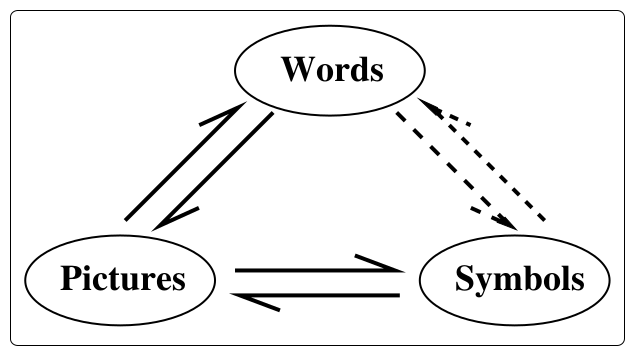
\includegraphics[scale=0.5]{imagens/palavras-imagens-simbolos.png}}
    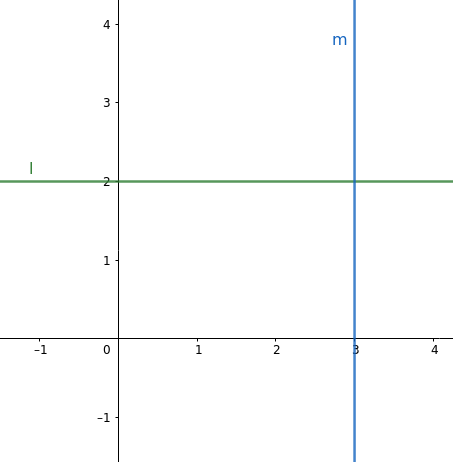
\includegraphics[scale=0.5]{imagens/curvas-simples.png}
    
    %\footnotesize{Fonte:~Precalculus}
  \end{center}
\end{figure}

A linha horizontal $l$ é descrita pela equação:

\begin{equation}
  \begin{split}
               l & = \left\{(x, k) | x \in \mathbb{R}, k \in \mathbb{R}, k = \text{constante}\right\}\\
                 & \therefore y = k
  \end{split}
\end{equation}

A linha vertical $m$ é descrita pela equação:

\begin{equation}
  \begin{split}
               m & = \left\{(h, y) | h \in \mathbb{R}, y \in \mathbb{R}, h = \text{constante}\right\}\\
                 & \therefore x = h
  \end{split}
\end{equation}


%%%%%%%%%%%%%%%%%%%%%%%%%%%%%%%%%%%%%%%%%%%%%%%%%%%%%%%%%%%%%%%%%%%%%%%%%%%%%%%%%
%%%%%%%%%%%%%%%%%%%%%%%%%%%%%%%%%%%%%%%%%%%%%%%%%%%%%%%%%%%%%%%%%%%%%%%%%%%%%%%%%
\subsection{Círculos}
\label{tres-curvas-circulos}

Um círculo no plano é uma curva se, e apenas se, a distância de todos os pontos
$(x, y)$ da curva à origem $(h, k)$ for a mesma. Note que essa distância é o raio $r$
do círculo.

\begin{figure}[ht]
  \begin{center}
    \caption{A terceira curva simples é o círculo}
    \label{fig:curvas-circulo}
    %\fbox{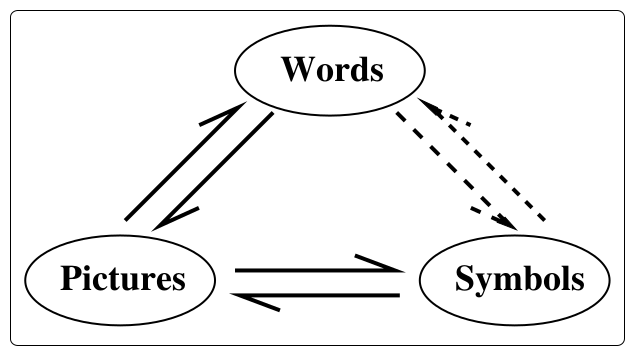
\includegraphics[scale=0.5]{imagens/palavras-imagens-simbolos.png}}
    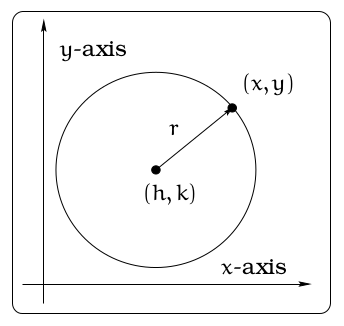
\includegraphics[scale=0.7]{imagens/definicao-circulo.png}
    
    \footnotesize{Fonte:~Collingwood DH et al. Precalculus, pág.\ 27}
  \end{center}
\end{figure}

O círculo é definido por:

\begin{equation}
  \begin{split}
    \text{Círculo} = \left\{(x, y) | x \in \mathbb{R}, y \in \mathbb{R}, \forall x \forall y\ r^2 = (|\Delta x|)^2 + (|\Delta y|)^2\right\}
  \end{split}
\end{equation}

A distância de qualquer ponto $(x, y)$, no círculo, à origem no ponto $(h, k)$, é o raio $r$ desse círculo
e é dado por:

\begin{equation}
  \begin{split}
    r^2 & = (|\Delta x|)^2 + (|\Delta y|)^2\\
        & = (|x - h|)^2 + (|y - k|)^2\\
      r & = \sqrt{(|x - h|)^2 + (|y - k|)^2}
  \end{split}
\end{equation}

Existe um caso especial que ocorre quando a origem do círculo estiver no ponto $(0, 0)$: nessa
situação o cálculo do raio $r$ simplifica-se por:

\begin{equation}
  \begin{split}
    r^2 & = (|\Delta x|)^2 + (|\Delta y|)^2\\
        & = (|x - h|)^2 + (|y - k|)^2\\
        & = (|x - 0|)^2 + (|y - 0|)^2\\
        & = (|x|)^2 + (|y|)^2\\
      r & = \sqrt{(|x|)^2 + (|y|)^2}
  \end{split}
\end{equation}

Um círculo de especial interesse matemático é o \emph{Círculo Unitário}, que é aquele
que tem origem em $(0, 0)$ e raio igual a 1 unidade:

\begin{equation}
  \begin{split}
    \text{Círculo Unitário} = \left\{(x, y) | x,y \in \mathbb{R}, \forall x \forall y\ r^2 = (|\Delta x|)^2 + (|\Delta y|)^2 = 1\right\}
  \end{split}
\end{equation}


%%%%%%%%%%%%%%%%%%%%%%%%%%%%%%%%%%%%%%%%%%%%%%%%%%%%%%%%%%%%%%%%%%%%%%%%%%%%%%%%%
%%%%%%%%%%%%%%%%%%%%%%%%%%%%%%%%%%%%%%%%%%%%%%%%%%%%%%%%%%%%%%%%%%%%%%%%%%%%%%%%%
\subsection{Cruzamento de curvas --- I}
\label{tres-curvas-cruzamento-I}

Obviamente, curvas horizontais não se cruzam (da mesma forma que
curvas verticais também não se cruzam).

Uma curva horizontal e uma curva vertical se cruzam apenas 1 única vez.
Já curvas horizontais ou verticais podem cruzar ou não um círculo em diferentes
situações: a) não cruzar o círculo; b) cruzar em apenas 1 ponto (a curva é uma tangente
ao círculo) ou c) cruzar em 2 pontos (a curva é uma secante ao círculo).

\begin{figure}[ht]
  \begin{center}
    \caption{Cruzamento de curvas}
    \label{fig:curvas-cruzamento-1}
    %\fbox{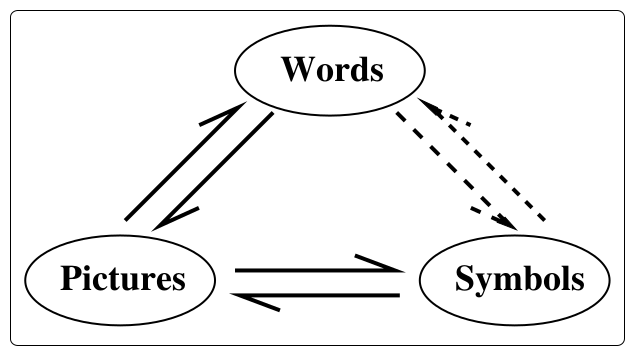
\includegraphics[scale=0.5]{imagens/palavras-imagens-simbolos.png}}
    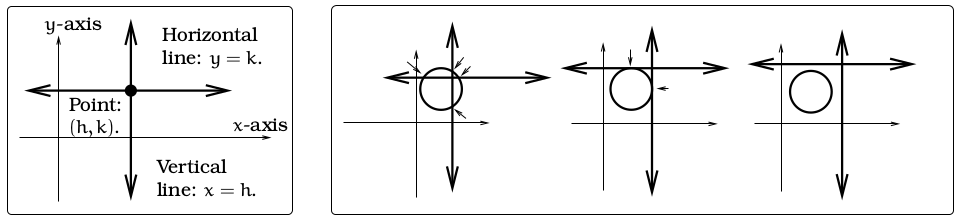
\includegraphics[scale=0.6]{imagens/cruzamento-curvas-1.png}
    
    \footnotesize{Fonte:~Collingwood DH et al. Precalculus, pág.\ 29}
  \end{center}
\end{figure}

O modo geral de se encontrar o ponto P onde as curvas de cruzam é resolver um
sistema de equações, uma para cada curva, e simultaneamente resolver ambas as
equações.


%%%%%%%%%%%%%%%%%%%%%%%%%%%%%%%%%%%%%%%%%%%%%%%%%%%%%%%%%%%%%%%%%%%%%%%%%%%%%%%%%
%%%%%%%%%%%%%%%%%%%%%%%%%%%%%%%%%%%%%%%%%%%%%%%%%%%%%%%%%%%%%%%%%%%%%%%%%%%%%%%%%
%%%%%%%%%%%%%%%%%%%%%%%%%%%%%%%%%%%%%%%%%%%%%%%%%%%%%%%%%%%%%%%%%%%%%%%%%%%%%%%%%
\section{Modelagem linear}
\label{modelagem-linear}

%%%%%%%%%%%%%%%%%%%%%%%%%%%%%%%%%%%%%%%%%%%%%%%%%%%%%%%%%%%%%%%%%%%%%%%%%%%%%%%%%
%%%%%%%%%%%%%%%%%%%%%%%%%%%%%%%%%%%%%%%%%%%%%%%%%%%%%%%%%%%%%%%%%%%%%%%%%%%%%%%%%
\subsection{Relacionando linhas e equações}
\label{modelagem-linear-relacionando-linhas}

Já temos as equações para linhas horizontais e verticais. Relembrando, para linhas horizontais
a equação é:

\begin{equation}
  \begin{split}
               l & = \left\{(x, k) | x \in \mathbb{R}, k \in \mathbb{R}, k = \text{constante}\right\}\\
                 & \therefore y = k
  \end{split}
\end{equation}

Para linhas verticais, a equação é:

\begin{equation}
  \begin{split}
               m & = \left\{(h, y) | h \in \mathbb{R}, y \in \mathbb{R}, h = \text{constante}\right\}\\
                 & \therefore x = h
  \end{split}
\end{equation}

O problema é: qual a equação para \emph{linhas INCLINADAS não verticais}? A equação desse tipo de linha é uma
das mais importantes na matemática pois é a base para muitas outras coisas. Lembre-se
de que 2 pontos diferentes completamente determinam uma linha reta.

%%%%%%%%%%%%%%%%%%%%%%%%%%%%%%%%%%%%%%%%%%%%%%%%%%%%%%%%%%%%%%%%%%%%%%%%%%%%%%%%%
%%%%%%%%%%%%%%%%%%%%%%%%%%%%%%%%%%%%%%%%%%%%%%%%%%%%%%%%%%%%%%%%%%%%%%%%%%%%%%%%%
\subsection{Linhas não verticais}
\label{modelagem-linear-linhas-nao-verticais}

A primeira coisa a determinar quando estamos tratando de uma linha não vertical,
é seu \textbf{\emph{slope}} (sua inclinação), comumente representado pela letra $m$. Por
exemplo, dados os pontos $P1 = (x_1, y_1)$ e $P2 = (x_2, y_2)$, o slope é:

\begin{equation}
  \begin{split}
    \text{Slope} = m & = \frac{\Delta y}{\Delta x}\\
                     & = \frac{y_2 - y_1}{x_2 - x_1}
  \end{split}
\end{equation}

O slope pode assumir diferentes valores:

\begin{itemize}[noitemsep]
\item Positivo: y aumenta a medida que x aumenta;
\item Negativo: y diminui a medida que x aumenta;
\item Zero: y permanece o mesmo a medida que x aumenta (linha horizontal)
\end{itemize}

Note que linhas verticais ($x = h$), por definição, não têm slope definido na matemática pois
$\Delta x = 0$ e $m = \frac{\Delta y}{0}$, que não é definido.

A partir do \emph{slope} e da informação sobre um ou mais pontos,
podemos determinar a equação para linhas não verticais de 3 modos diferentes! Considere que:

\begin{itemize}
\item $\bm{P=(x,y)}$ é um ponto arbitrário qualquer na linha (não sabemos o valor de x ou y);
\item $\bm{Q=(x_0, y_0)}$ é um ponto conhecido, ou seja, sabemos o valor de x ($x_0$) e o valor de y ($y_0$);
\item $\bm{R=(x_1,y_2)}$ é outro ponto conhecido, ou seja, sabemos o valor de x ($x_1$) e o valor de y ($y_1$); e
\item $\bm{m}$ é o slope da linha.
\end{itemize}

Se soubermos o valor de $m$ e de algum ponto $Q=(x_0, y_0)$, podemos definir a
\textbf{Equação POINT-SLOPE} da linha para qualquer ponto desconhecido $P=(x,y)$:

\begin{equation}
  \begin{split}
    m & = \frac{\Delta y}{\Delta x}\\
    m & = \frac{y - y_0}{x - x_0}\\
    m(x - x_0) & = y - y_0\\
    y - y_0 & = m(x - x_0)\\
    \bm{\therefore y} & \bm{= m(x-x_0) + y_0}
  \end{split}
\end{equation}

Se soubermos o valor de dois pontos, $Q=(x_0, y_0)$ e $R=(x_1, y_1)$, podemos definir
a \textbf{Equação TWO-POINT} da linha para qualquer ponto desconhecido $P=(x, y)$:

\begin{equation}
  \begin{split}
    m & = \frac{\Delta y}{\Delta x}\\
    m & = \frac{y_1 - y_0}{x_1 - x_0}\\
      & \therefore\\
    y - y_0 & = \left(\frac{y_1 - y_0}{x_1 - x_0}\right)(x - x_0)\\
    \bm{\therefore y} & \bm{= \left(\frac{y_1 - y_0}{x_1 - x_0}\right)(x-x_0) + y_0}
  \end{split}
\end{equation}

Se soubermos o valor de $m$ e de algum ponto $Q=(x_0, y_0)$, e se essa linha cruzar
o eixo-y nesse ponto (portanto $x_0 = 0$ e $y_0 = \text{intercepto-y}$), podemos definir a
\textbf{Equação SLOPE-INTERCEPT} da linha para qualquer ponto
desconhecido $P=(x, y)$:

\begin{equation}
  \begin{split}
    m & = \frac{\Delta y}{\Delta x}\\
    m & = \frac{y - y_0}{x - x_0}\\
    m & = \frac{y - y_0}{x - 0}\\
    m & = \frac{y - y_0}{x}\\
    m(x) & = y - y_0\\
    y - y_0 & = mx\\
    \bm{\therefore y} & \bm{= mx + y_0}
  \end{split}
\end{equation}

Em resumo, até agora, já vimos 3 equações para linhas não verticais:

\begin{itemize}
\item \textbf{Equação POINT-SLOPE}: define a linha com $m$ e um ponto conhecido:

  $y = m(x - x_0) + y_0$
\item \textbf{Equação TWO-POINT}: define a linha com 2 pontos:

  $y = \left(\frac{y_1 - y_0}{x_1 - x_0}\right)(x - x_0) + y_0$
\item \textbf{Equação SLOPE-INTERCEPT}: define a linha com $m$ e intercepto-y:

  $y = mx + y_0$
\end{itemize}

%%%%%%%%%%%%%%%%%%%%%%%%%%%%%%%%%%%%%%%%%%%%%%%%%%%%%%%%%%%%%%%%%%%%%%%%%%%%%%%%%
%%%%%%%%%%%%%%%%%%%%%%%%%%%%%%%%%%%%%%%%%%%%%%%%%%%%%%%%%%%%%%%%%%%%%%%%%%%%%%%%%
\subsection{Linhas em geral}
\label{modelagem-linear-linhas-gerais}

Além das 3 equações anteriores para linhas não verticais, qualquer linha no
plano pode ser obtida através da \textbf{Equação LINEAR GERAL} (sendo A, B e C constantes)\footnote{A equação
  linear geral serve para linhas em mais de dois planos, por exemplo: em um sistema de coordenadas
  tri-dimensional, a equação linear geral é $Ax + By + Cz + D = 0$, com A, B, C e D constantes.}:

\begin{equation}
  Ax + By + C = 0
\end{equation}

Essa equação linear geral no plano pode ser derivada,
a partir de 2 pontos $P=(x_0, y_0)$ e $Q=(x_1, y_1)$ da seguinte maneira:

\begin{equation}
  \begin{split}
    m & = \frac{y_1 - y_0}{x_1 - x_0}\\
      & \therefore\\
    y - y_0 & = \frac{y_1 - y_0}{x_1 - x_0}(x - x_0)\\
    (y - y_0)(x_1 - x_0) & = (y_1 - y_0)(x - x_0)\\
    x_1y - x_0y - x_1y_0 + x_0y_0 & = xy_1 - x_0y_1 - xy_0 + x_0y_0\\
    x_1y - x_0y - x_1y_0 + \cancel{x_0y_0} & = xy_1 - x_0y_1 - xy_0 + \cancel{x_0y_0}\\
    xy_1 - x_0y_1 - xy_0 & = x_1y - x_0y - x_1y_0\\
    xy_1 - x_0y_1 - xy_0 - x_1y + x_0y + x_1y_0 & = 0\\
    xy_1 - xy_0 + x_0y - x_1y + x_1y_0 - x_0y_1 & = 0\\
    & \therefore\\
    \bm{(y_1 - y_0)x + (x_0 - x_1)y + (x_1y_0 - x_0y_1)} &\bm{= 0}
  \end{split}
\end{equation}

A equação linear geral pode ser utilizada para definir uma linha vertical, ao contrário
das outras equações que já vimos. Por exemplo: $-4x + 0y + 12 = 0$ define uma linha vertical
com $x = 3$.

Propriedades da equação linear geral:

\begin{itemize}
\item Slope: $-\frac{A}{B}$
\item Intercepto-y: $-\frac{C}{B}$
\item Intercepto-x: $-\frac{C}{A}$
\item Se $B = 0$, linha é vertical e slope não é definido (intercepto-y também não faz sentido)
\item Se $B \neq 0$, linha não é vertical
\end{itemize}

As propriedades da equação linear geral listadas acima podem ser derivadas através de
simples manipulações algébricas:

\begin{equation}
  \begin{split}
    Ax + By + C & = 0\\
    By & = -Ax -C\\
    y & = \frac{-Ax -C}{B}\\
    \bm{y} & \bm{= -\frac{A}{B}x -\frac{C}{B}}\\
    & \therefore\\
    \text{slope} & = -\frac{A}{B}\\
    \text{intercepto-y} & = -\frac{C}{B}\\
    \text{intercepto-x} & = -\frac{C}{A}
  \end{split}
\end{equation}


%%%%%%%%%%%%%%%%%%%%%%%%%%%%%%%%%%%%%%%%%%%%%%%%%%%%%%%%%%%%%%%%%%%%%%%%%%%%%%%%%
%%%%%%%%%%%%%%%%%%%%%%%%%%%%%%%%%%%%%%%%%%%%%%%%%%%%%%%%%%%%%%%%%%%%%%%%%%%%%%%%%
\subsection{Linhas e taxas de variação}
\label{modelagem-linear-linhas-taxa-variacao}

Já deve estar bem claro que, para linhas não verticais, o slope da linha corresponde
à taxa de variação de $y$ em relação à $x$, sendo essa taxa constante.

Se $x$ for
uma medida de tempo, o slope fornecerá uma taxa muito comum e importante: a \emph{velocidade}:

\begin{equation}
  \text{velocidade} = \frac{\Delta y}{\Delta x} = \frac{\Delta y}{\Delta \text{tempo}}
\end{equation}

Assim, a equação para a localização de um objeto que se move a uma velocidade constante
($m$ = velocidade; $x$ = tempo; $y_0$ = posição inicial), é dada por:

\begin{equation}
  \begin{split}
    y & = mx + y_0\\
    y & = vt + y_0
  \end{split}
\end{equation}


%%%%%%%%%%%%%%%%%%%%%%%%%%%%%%%%%%%%%%%%%%%%%%%%%%%%%%%%%%%%%%%%%%%%%%%%%%%%%%%%%
%%%%%%%%%%%%%%%%%%%%%%%%%%%%%%%%%%%%%%%%%%%%%%%%%%%%%%%%%%%%%%%%%%%%%%%%%%%%%%%%%
\subsection{O que é necessário para construir um modelo linear?}
\label{modelagem-linear-necessario-para-modelo}

Conforme percebemos por todas as equações das linhas que estudamos até agora,
para se definir um modelo, uma equação linear, sempre precisamos de DUAS INFORMAÇÕES:

\begin{itemize}[noitemsep]
\item Um ponto e um slope; ou
\item Dois pontos; ou
\item Um slope e um intercepto-y.
\end{itemize}


%%%%%%%%%%%%%%%%%%%%%%%%%%%%%%%%%%%%%%%%%%%%%%%%%%%%%%%%%%%%%%%%%%%%%%%%%%%%%%%%%
%%%%%%%%%%%%%%%%%%%%%%%%%%%%%%%%%%%%%%%%%%%%%%%%%%%%%%%%%%%%%%%%%%%%%%%%%%%%%%%%%
\subsection{Linhas paralelas e perpendiculares}
\label{modelagem-linear-paralelas-perpendiculares}

Duas linhas não verticias podem se cruzar em diversos ângulos, mas 2 situações
são especiais.

O primeiro caso é quando duas linhas, 1 e 2, são paralelas. Nessa situação,
o slope das linhas será igual:

\begin{equation}
  \text{Linhas Paralelas} \equiv m_1 = m_2
\end{equation}

O segundo caso é quando duas linhas, 1 e 2, são perpendiculares. Nessa situação
o slope de uma será o inverso negativo da outra:

\begin{equation}
  \begin{split}
    \text{Linhas Perpendiculares} \equiv m_1    & = -\frac{1}{m_2}\\
                                         m_1m_2 & = -1
  \end{split}
\end{equation}


%%%%%%%%%%%%%%%%%%%%%%%%%%%%%%%%%%%%%%%%%%%%%%%%%%%%%%%%%%%%%%%%%%%%%%%%%%%%%%%%%
%%%%%%%%%%%%%%%%%%%%%%%%%%%%%%%%%%%%%%%%%%%%%%%%%%%%%%%%%%%%%%%%%%%%%%%%%%%%%%%%%
\subsection{Cruzamento de curvas --- II}
\label{modelagem-linear-cruzamento-curvas-ii}

Já vimos que para resolver problemas que envolvem o cruzamento de linhas ou
de linhas com curvas (círculos, por exemplo), temos que trabalhar com um sistema
de equações com as variáveis x e y.

Frequentemente a fórmula quadrática ($ax^2 + bx + c = 0$) será necessária. A
solução da fórmula quadrática é dada por:

\begin{equation}
  x = \frac{-(b) \pm \sqrt{(b)^2 - (4ac)}}{2a}
\end{equation}

As duas raízes encontradas, $x'$ e $x''$, indicam em que valores no eixo-x a
curva do círculo se cruza com esse eixo.

%%%%%%%%%%%%%%%%%%%%%%%%%%%%%%%%%%%%%%%%%%%%%%%%%%%%%%%%%%%%%%%%%%%%%%%%%%%%%%%%%
%%%%%%%%%%%%%%%%%%%%%%%%%%%%%%%%%%%%%%%%%%%%%%%%%%%%%%%%%%%%%%%%%%%%%%%%%%%%%%%%%
\subsection{Movimento linear uniforme}
\label{modelagem-linear-movimento-uniforme}

Quando um objeto se move ao longo de uma linha em um plano a uma velocidade constante,
dizemos que ele está em \emph{movimento linear uniforme}.

Nessa situação, se
conhecermos a localização do objeto em 2 pontos no tempo, podemos substituir a equação
linear que envolve 2 variáveis (x e y) por um sistema de equações que envolve somente 1
variável (t = tempo). Esse sistema de equações é dado por:

\begin{equation}
  \begin{split}
    x &= a + bt\\
    y &= c + dt
  \end{split}
\end{equation}

Esse sistema de equações é chamado de \emph{Equações Paramétricas do Movimento} e só
depende do parâmetro t (tempo), com A, B, C e D constantes.


%%%%%%%%%%%%%%%%%%%%%%%%%%%%%%%%%%%%%%%%%%%%%%%%%%%%%%%%%%%%%%%%%%%%%%%%%%%%%%%%%
%%%%%%%%%%%%%%%%%%%%%%%%%%%%%%%%%%%%%%%%%%%%%%%%%%%%%%%%%%%%%%%%%%%%%%%%%%%%%%%%%
%%%%%%%%%%%%%%%%%%%%%%%%%%%%%%%%%%%%%%%%%%%%%%%%%%%%%%%%%%%%%%%%%%%%%%%%%%%%%%%%%
\section{Funções e gráficos}
\label{funcoes-graficos}

%%%%%%%%%%%%%%%%%%%%%%%%%%%%%%%%%%%%%%%%%%%%%%%%%%%%%%%%%%%%%%%%%%%%%%%%%%%%%%%%%
%%%%%%%%%%%%%%%%%%%%%%%%%%%%%%%%%%%%%%%%%%%%%%%%%%%%%%%%%%%%%%%%%%%%%%%%%%%%%%%%%
\subsection{Relacionando dados, plots (traçados) e equações}
\label{funcoes-graficos-relacionando}

Existem 3 maneiras de descrevermos o relacionamento entre uma variável $y$ à
outra variável $x$:

\begin{itemize}[noitemsep]
\item Uma tabela
\item Um gráfico
\item Uma equação
\end{itemize}

A partir da tabela de dados podemos plotar um gráfico em um sistema de coordenadas
e, a partir desse gráfico (ou desses dados), podemos realizar uma \emph{modelagem}
para obtermos uma \emph{equação} que relacione $y$ à $x$:

\begin{figure}[ht]
  \begin{center}
    \caption{Relação entre dados, plots e equações}
    \label{fig:relacao-dados-plots-equacoes}
    %\fbox{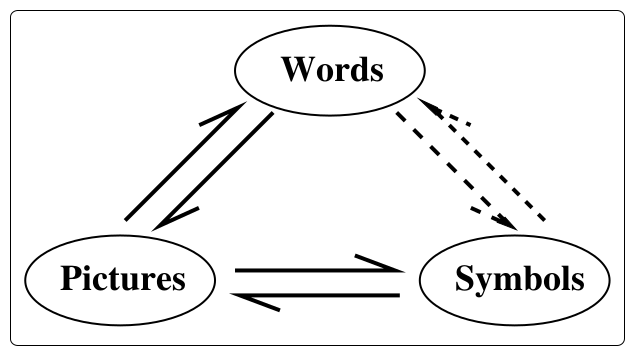
\includegraphics[scale=0.5]{imagens/palavras-imagens-simbolos.png}}
    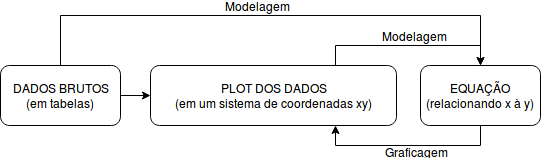
\includegraphics[scale=0.7]{imagens/relacao_dados_plot_equacao.png}
    
    %\footnotesize{Fonte:~Collingwood DH et al. Precalculus, pág.\ 29}
  \end{center}
\end{figure}

Obviamente a equação é muito mais poderosa do que somente a tabela de dados, pois
ela nos mostra exatamente como $y$ varia \emph{em função} de $x$. Agora temos
um outro conceito importante, o conceito de FUNÇÃO!


%%%%%%%%%%%%%%%%%%%%%%%%%%%%%%%%%%%%%%%%%%%%%%%%%%%%%%%%%%%%%%%%%%%%%%%%%%%%%%%%%
%%%%%%%%%%%%%%%%%%%%%%%%%%%%%%%%%%%%%%%%%%%%%%%%%%%%%%%%%%%%%%%%%%%%%%%%%%%%%%%%%
\subsection{O que é uma função?}
\label{funcoes-conceito}

Uma função é uma \emph{regra} (equação) que nos informa como relacionar cada elemento
de um conjunto de inputs aceitáveis (\emph{domínio}, D) a um, e somente um,
elemento de um conjunto de outputs (\emph{codomínio} ou \emph{range} R).

\begin{figure}[H]
  \begin{center}
    \caption{Esquema de uma função}
    \label{fig:esquema-funcao}
    %\fbox{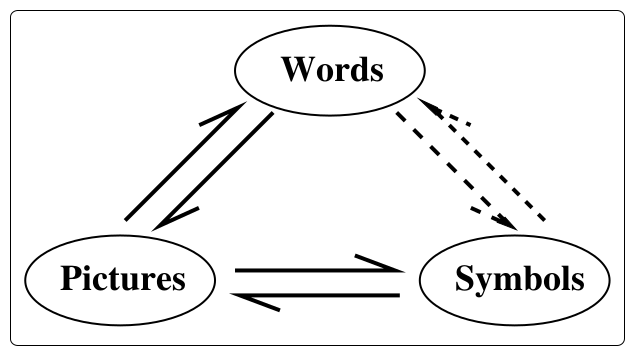
\includegraphics[scale=0.5]{imagens/palavras-imagens-simbolos.png}}
    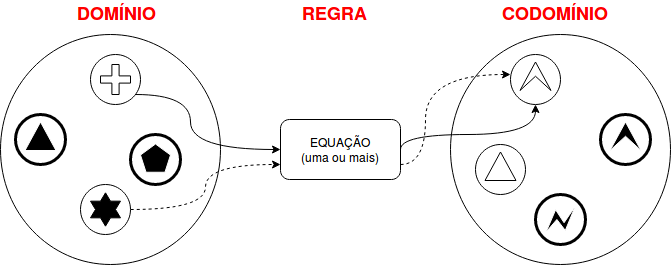
\includegraphics[scale=0.5]{imagens/esquema-funcao.png}
    
    %\footnotesize{Fonte:~Collingwood DH et al. Precalculus, pág.\ 29}
  \end{center}
\end{figure}

Note que cada elemento do domínio deve estar relacionado a um, e apenas um,
elemento do range, mas o mesmo elemento do range pode estar relacionado a
mais de um elemento do domínio. Se um elemento do domínio estiver relacionado
a mais de um elemento do codomínio, a regra em questão não é uma função!

Uma função sempre tem 3 partes:

\begin{itemize}
\item \textbf{DOMÍNIO}: é o conjunto de inputs aceitáveis:

  $D = \left\{x\ |\ x\ \text{é aceitável}\right\}$
\item \textbf{REGRA}: é a regra (geralmente na forma de uma ou mais equações)
  que informa como relacionar os elementos do domínio aos elementos do range.
  As regras são identificadas por letras (f, g, h, \ldots):

  $f(x) = \text{equação}$
\item \textbf{RANGE ou CODOMÍNIO}: é o conjunto de outputs:

  $R = \left\{f(x)\ |\ f(x)\ \text{é único para cada }x\right\}$
\end{itemize}

Note a diferença na notação:

\begin{itemize}[noitemsep]
\item $f(x)$: refere-se à \emph{regra} da função;
\item $y = f(x)$: refere-se à função em si, ou seja, estamos dizendo que $y$ varia
  em função de $x$ através da regra $f$.
\end{itemize}

A \emph{especificação completa} de uma função é dada pela regra e pelo domínio
aceitável:

\begin{equation}
    y = f(x) = ax + b \quad |\ D = \left\{x\ |\ x \in \mathbb{R}\right\}
\end{equation}

Dependendo do domínio aceitável, uma mesma regra pode definir funções diferentes.
Nesse caso, usamos letras diferentes:

\begin{equation}
  \begin{split}
    y & = f(x) = ax + b \quad |\ D = \left\{x\ |\ x \in \mathbb{R}\right\}\\
    y & = g(x) = ax + b \quad |\ D = \left\{x\ |\ x \in \mathbb{R}, x \ge 0\right\}
  \end{split}
\end{equation}

Ainda em relação ao domínio de uma função, ele pode ser:

\begin{itemize}[noitemsep]
\item Toda linha numérica
\item Um intervalo da linha numérica, incluindo ou não os pontos extremos desse intervalo:
  $[a,b]$, $(a,b]$, $[a,b)$, $(a,b)$
\item Um conjunto finito de intervalos da linha linha numérica (também incluindo ou não os pontos extremos desses intervalos)
\end{itemize}


%%%%%%%%%%%%%%%%%%%%%%%%%%%%%%%%%%%%%%%%%%%%%%%%%%%%%%%%%%%%%%%%%%%%%%%%%%%%%%%%%
%%%%%%%%%%%%%%%%%%%%%%%%%%%%%%%%%%%%%%%%%%%%%%%%%%%%%%%%%%%%%%%%%%%%%%%%%%%%%%%%%
\subsection{Gráfico de uma função}
\label{funcoes-grafico}

Já vimos que para especificarmos uma função $y = f(x)$, além da regra $f$ temos que
especificar o domínio $D$. Ao especificarmos a regra e o domínio, o gráfico de
uma função será o conjunto de pontos $(x, f(x))$ para todo $x \in D$.


%%%%%%%%%%%%%%%%%%%%%%%%%%%%%%%%%%%%%%%%%%%%%%%%%%%%%%%%%%%%%%%%%%%%%%%%%%%%%%%%%
%%%%%%%%%%%%%%%%%%%%%%%%%%%%%%%%%%%%%%%%%%%%%%%%%%%%%%%%%%%%%%%%%%%%%%%%%%%%%%%%%
\subsection{O teste da linha vertical}
\label{funcoes-teste-linha-vertical}

Ao analisarmos o gráfico de alguma curva, podemos dizer facilmente se essa curva
é, ou não, o gráfico de uma função.

Já que uma função produz um, e apenas um, output para cada input, se uma linha
vertical (perpendicular) ao eixo-x cruzar a curva em 2 ou mais pontos,
essa curva NÃO é uma função (pois isso implica em dizer que há mais de um codomínio
para cada elemento do domínio).

%%%%%%%%%%%%%%%%%%%%%%%%%%%%%%%%%%%%%%%%%%%%%%%%%%%%%%%%%%%%%%%%%%%%%%%%%%%%%%%%%
%%%%%%%%%%%%%%%%%%%%%%%%%%%%%%%%%%%%%%%%%%%%%%%%%%%%%%%%%%%%%%%%%%%%%%%%%%%%%%%%%
\subsection{Funções lineares}
\label{funcoes-lineares}

A equação da linha reta não vertical, que já conhecemos, é, na verdade,
uma função: $y = f(x) = mx + b$.

Um dos principais conteúdos do pré-cálculo é o estudo de diversas funções pois
as funções são fundamentais no cálculo.




%%%%%%%%%%%%%%%%%%%%%%%%%%%%%%%%%%%%%%%%%%%%%%%%%%%%%%%%%%%%%%%%%%%%%%%%%%%%%%%%%
%%%%%%%%%%%%%%%%%%%%%%%%%%%%%%%%%%%%%%%%%%%%%%%%%%%%%%%%%%%%%%%%%%%%%%%%%%%%%%%%%
%%%%%%%%%%%%%%%%%%%%%%%%%%%%%%%%%%%%%%%%%%%%%%%%%%%%%%%%%%%%%%%%%%%%%%%%%%%%%%%%%
\section{Análise gráfica}
\label{analise-grafica}

%%%%%%%%%%%%%%%%%%%%%%%%%%%%%%%%%%%%%%%%%%%%%%%%%%%%%%%%%%%%%%%%%%%%%%%%%%%%%%%%%
%%%%%%%%%%%%%%%%%%%%%%%%%%%%%%%%%%%%%%%%%%%%%%%%%%%%%%%%%%%%%%%%%%%%%%%%%%%%%%%%%
\subsection{Análise visual de um gráfico}
\label{analise-grafica-visual}

Ao realizar a análise de um gráfico de uma função, temos que procurar pelas suas
6 características qualitativas básicas:

\begin{enumerate}
\item \textbf{Domínio} e \textbf{Range}: qual o domínio e o range da função?
\item \textbf{Sign Plot}: em quais segmentos $y = f(x)$ é positiva ou negativa?
\item \textbf{Dinâmica Visual}: como $f(x)$ varia em função de $x$? Em que segmentos
  $f(x)$ aumenta, diminui ou permanece constante em relação à $x$?
\item \textbf{Y-intercepto}: em que valor de $x$ a função cruza o eixo-y? Note
  que, uma função, só cruza o eixo-y em no máximo 1 único local. Assim, uma função
  pode não ter intercepto-y, ou pode ter apenas 1 único intercepto-y.
\item \textbf{X-intercepto}: em que locais a curva da função cruza o eixo-y? Note
  que uma função pode não cruzar o eixo-x, ou cruzá-lo em 1 ou vários pontos. Cada
  ponto onde a curva cruza o eixe-x são os ``zeros'' ou ``raízes'' da função $y=f(x)$.
\item \textbf{Máximos} e \textbf{Mínimos ``locais''}: são os pontos onde a função ``pára''
  na curva (no topo de um morro ou no fundo de uma depressão).
\end{enumerate}


%%%%%%%%%%%%%%%%%%%%%%%%%%%%%%%%%%%%%%%%%%%%%%%%%%%%%%%%%%%%%%%%%%%%%%%%%%%%%%%%%
%%%%%%%%%%%%%%%%%%%%%%%%%%%%%%%%%%%%%%%%%%%%%%%%%%%%%%%%%%%%%%%%%%%%%%%%%%%%%%%%%
\subsection{Círculos e semi-círculos}
\label{analise-grafica-circulos}

Já sabemos que um círculo é uma curva onde a distância de qualquer ponto $(x,y)$
à origem $(h,k)$ é a mesma, ou seja, é $r$ (o raio):

\begin{equation}
  \text{Círculo} = \left\{(x,y)\ |\ x,y \in \mathbb{R}, \forall x \forall y\ r^2 = (|\Delta x|)^2 + (|\Delta y|)^2 = \text{constante}\right\}
\end{equation}

Na equação do círculo, $\Delta x = x - h$ e $\Delta y = y - k$. Note que a equação do círculo não é uma função, pois
para cada valor de $x$ existem 2 valores $f(x)$. Mas podemos obter 2 funções correspondentes
aos semi-círculos: superior e inferior!

\begin{equation}
  \begin{split}
    r^2 & = (|\Delta x|)^2 + (|\Delta y|)^2\\
    r^2 & = (x - h)^2 + (y - k)^2\\
    (y - k)^2 & = r^2 - (x - h)^2\\
    y - k & = \pm \sqrt{r^2 - (x - h)^2}\\
    \bm{y} & \bm{= k \pm \sqrt{r^2 - (x - h)^2}}
  \end{split}
\end{equation}

As equações das funções que representam cada semi-círculo são, então:
\begin{equation}
  \begin{split}
    y & = f(x) = k \bm{+} \sqrt{r^2 - (x - h)^2}\\
    y & = g(x) = k \bm{-} \sqrt{r^2 - (x - h)^2}
  \end{split}
\end{equation}


%%%%%%%%%%%%%%%%%%%%%%%%%%%%%%%%%%%%%%%%%%%%%%%%%%%%%%%%%%%%%%%%%%%%%%%%%%%%%%%%%
%%%%%%%%%%%%%%%%%%%%%%%%%%%%%%%%%%%%%%%%%%%%%%%%%%%%%%%%%%%%%%%%%%%%%%%%%%%%%%%%%
\subsection{Funções com múltiplas partes}
\label{analise-grafica-multipart}

Uma função $y=f(x)$ será uma função com múltiplas partes quando, em seu domínio,
existirem mais de uma regra $f(x)$:

\begin{equation}
  y = f(x) =
  \begin{cases} 
      1                & se\ x < -1 \\
      1 + \sqrt{1-x^2} & se\ -1 \leq x \leq 1 \\
      1                & se\ x > 1
  \end{cases}
\end{equation}

ATENÇÃO: em uma função com múltiplas partes temos que tera certeza de que essas
múltiplas partes, quando tomadas em conjunto, realmente formam um função, ou seja,
se realmente só haverá um único elemento no range para cada elemento do domínio.




%%%%%%%%%%%%%%%%%%%%%%%%%%%%%%%%%%%%%%%%%%%%%%%%%%%%%%%%%%%%%%%%%%%%%%%%%%%%%%%%%
%%%%%%%%%%%%%%%%%%%%%%%%%%%%%%%%%%%%%%%%%%%%%%%%%%%%%%%%%%%%%%%%%%%%%%%%%%%%%%%%%
%%%%%%%%%%%%%%%%%%%%%%%%%%%%%%%%%%%%%%%%%%%%%%%%%%%%%%%%%%%%%%%%%%%%%%%%%%%%%%%%%
\section{Modelagem quadrática}
\label{modelagem-quadratica}

%%%%%%%%%%%%%%%%%%%%%%%%%%%%%%%%%%%%%%%%%%%%%%%%%%%%%%%%%%%%%%%%%%%%%%%%%%%%%%%%%
%%%%%%%%%%%%%%%%%%%%%%%%%%%%%%%%%%%%%%%%%%%%%%%%%%%%%%%%%%%%%%%%%%%%%%%%%%%%%%%%%
\subsection{Parábolas e Vértice}
\label{modelagem-quadratica-parabolas}



%%%%%%%%%%%%%%%%%%%%%%%%%%%%%%%%%%%%%%%%%%%%%%%%%%%%%%%%%%%%%%%%%%%%%%%%%%%%%%%%%
%\subsubsection{Subsubseção}
%\label{subsubetiqueta}


%%%%%%%%%%%%%%%%%%%%%%%%%%%%%%%%%%%%%%%%%%%%%%%%%%%%%%%%%%%%%%%%%%%%%%%%%%%%%%%%%
%%%%%%%%%%%%%%%%%%%%%%%%%%%%%%%%%%%%%%%%%%%%%%%%%%%%%%%%%%%%%%%%%%%%%%%%%%%%%%%%%
%%%%%%%%%%%%%%%%%%%%%%%%%%%%%%%%%%%%%%%%%%%%%%%%%%%%%%%%%%%%%%%%%%%%%%%%%%%%%%%%%
%%%%%%%%%%%%%%%%%%%%%%%%%%%%%%%%%%%%%%%%%%%%%%%%%%%%%%%%%%%%%%%%%%%%%%%%%%%%%%%%%
%%%%%%%%%%%%%%%%%%%%%%%%%%%%%% TERMINA O DOCUMENTO %%%%%%%%%%%%%%%%%%%%%%%%%%%%%%
%%%%%%%%%%%%%%%%%%%%%%%%%%%%%%%%%%%%%%%%%%%%%%%%%%%%%%%%%%%%%%%%%%%%%%%%%%%%%%%%%
%%%%%%%%%%%%%%%%%%%%%%%%%%%%%%%%%%%%%%%%%%%%%%%%%%%%%%%%%%%%%%%%%%%%%%%%%%%%%%%%%
%%%%%%%%%%%%%%%%%%%%%%%%%%%%%%%%%%%%%%%%%%%%%%%%%%%%%%%%%%%%%%%%%%%%%%%%%%%%%%%%%
%%%%%%%%%%%%%%%%%%%%%%%%%%%%%%%%%%%%%%%%%%%%%%%%%%%%%%%%%%%%%%%%%%%%%%%%%%%%%%%%%
\end{document}









